\documentclass[9pt,twocolumn,twoside, lineno]{pnas-new}
% Use the lineno option to display guide line numbers if required.

\templatetype{pnasresearcharticle} % Choose template
% {pnasresearcharticle} = Template for a two-column research article
% {pnasmathematics} %= Template for a one-column mathematics article
% {pnasinvited} %= Template for a PNAS invited submission

\begin{document}


\title{Hot spot model of risk structured disease spread}

% Use letters for affiliations, numbers to show equal authorship (if applicable) and to indicate the corresponding author
\author[a,b,d]{Brendan Wallace}
\author[c,d]{Dobrimir Dimitrov}
\author[a,b]{Andrew Berdahl}

\affil[a]{Quantitative Ecology and Resource Management Program,
University of Washington, Seattle, WA 98195, USA (UW)}
\affil[b]{School of Aquatic and Fishery Sciences, UW}
\affil[c]{Vaccine and Infectious Disease Division, Fred Hutchinson Cancer Research Center, Seattle, 98195 WA, USA}
\affil[d]{Department of Applied Mathematics, UW}

% Please give the surname of the lead author for the running footer
\leadauthor{Wallace}

% Please add a significance statement to explain the relevance of your work
\significancestatement{Authors must submit a 120-word maximum statement about the significance of their research paper written at a level understandable to an undergraduate educated scientist outside their field of speciality. The primary goal of the significance statement is to explain the relevance of the work in broad context to a broad readership. The significance statement appears in the paper itself and is required for all research papers.}

% Please include corresponding author, author contribution and author declaration information
\authorcontributions{Please provide details of author contributions here.}
\authordeclaration{Please declare any competing interests here.}
\equalauthors{\textsuperscript{1}A.O.(Author One) contributed equally to this work with A.T. (Author Two) (remove if not applicable).}
\correspondingauthor{\textsuperscript{2}To whom correspondence should be addressed. E-mail: author.two\@email.com}

% At least three keywords are required at submission. Please provide three to five keywords, separated by the pipe symbol.
\keywords{Keyword 1 $|$ Keyword 2 $|$ Keyword 3 $|$ ...}

\begin{abstract}
Please provide an abstract of no more than 250 words in a single paragraph. Abstracts should explain to the general reader the major contributions of the article. References in the abstract must be cited in full within the abstract itself and cited in the text.
\end{abstract}

\dates{This manuscript was compiled on \today}
\doi{\url{www.pnas.org/cgi/doi/10.1073/pnas.XXXXXXXXXX}}


\maketitle
\thispagestyle{firststyle}
\ifthenelse{\boolean{shortarticle}}{\ifthenelse{\boolean{singlecolumn}}{\abscontentformatted}{\abscontent}}{}

\firstpage{7}
% Use \firstpage to indicate which paragraph and line will start the second page and subsequent formatting. In this example, there are a total of 11 paragraphs on the first page, counting the first level heading as a paragraph. The value {12} represents the number of the paragraph starting the second page. If a paragraph runs over onto the second page, include a bracket with the paragraph line number starting the second page, followed by the paragraph number in curly brackets, e.g. "\firstpage[4]{11}".


% % If your first paragraph (i.e. with the \dropcap) contains a list environment (quote, quotation, theorem, definition, enumerate, itemize...), the line after the list may have some extra indentation. If this is the case, add \parshape=0 to the end of the list environment.
% \dropcap{T}his PNAS journal template is provided to help you write your work in the correct journal format. Instructions for use are provided below.

% Note: please start your introduction without including the word ``Introduction'' as a section heading (except for math articles in the Physical Sciences section); this heading is implied in the first paragraphs.

% \subsection*{Manuscript Length}

% A standard 6-page article is approximately 4,000 words, 50 references, and 4 medium-size graphical elements (i.e., figures and tables). The preferred length of articles remains at 6 pages, but PNAS will allow articles up to a maximum of 12 pages.


% \begin{figure}%[tbhp]
% \centering
% 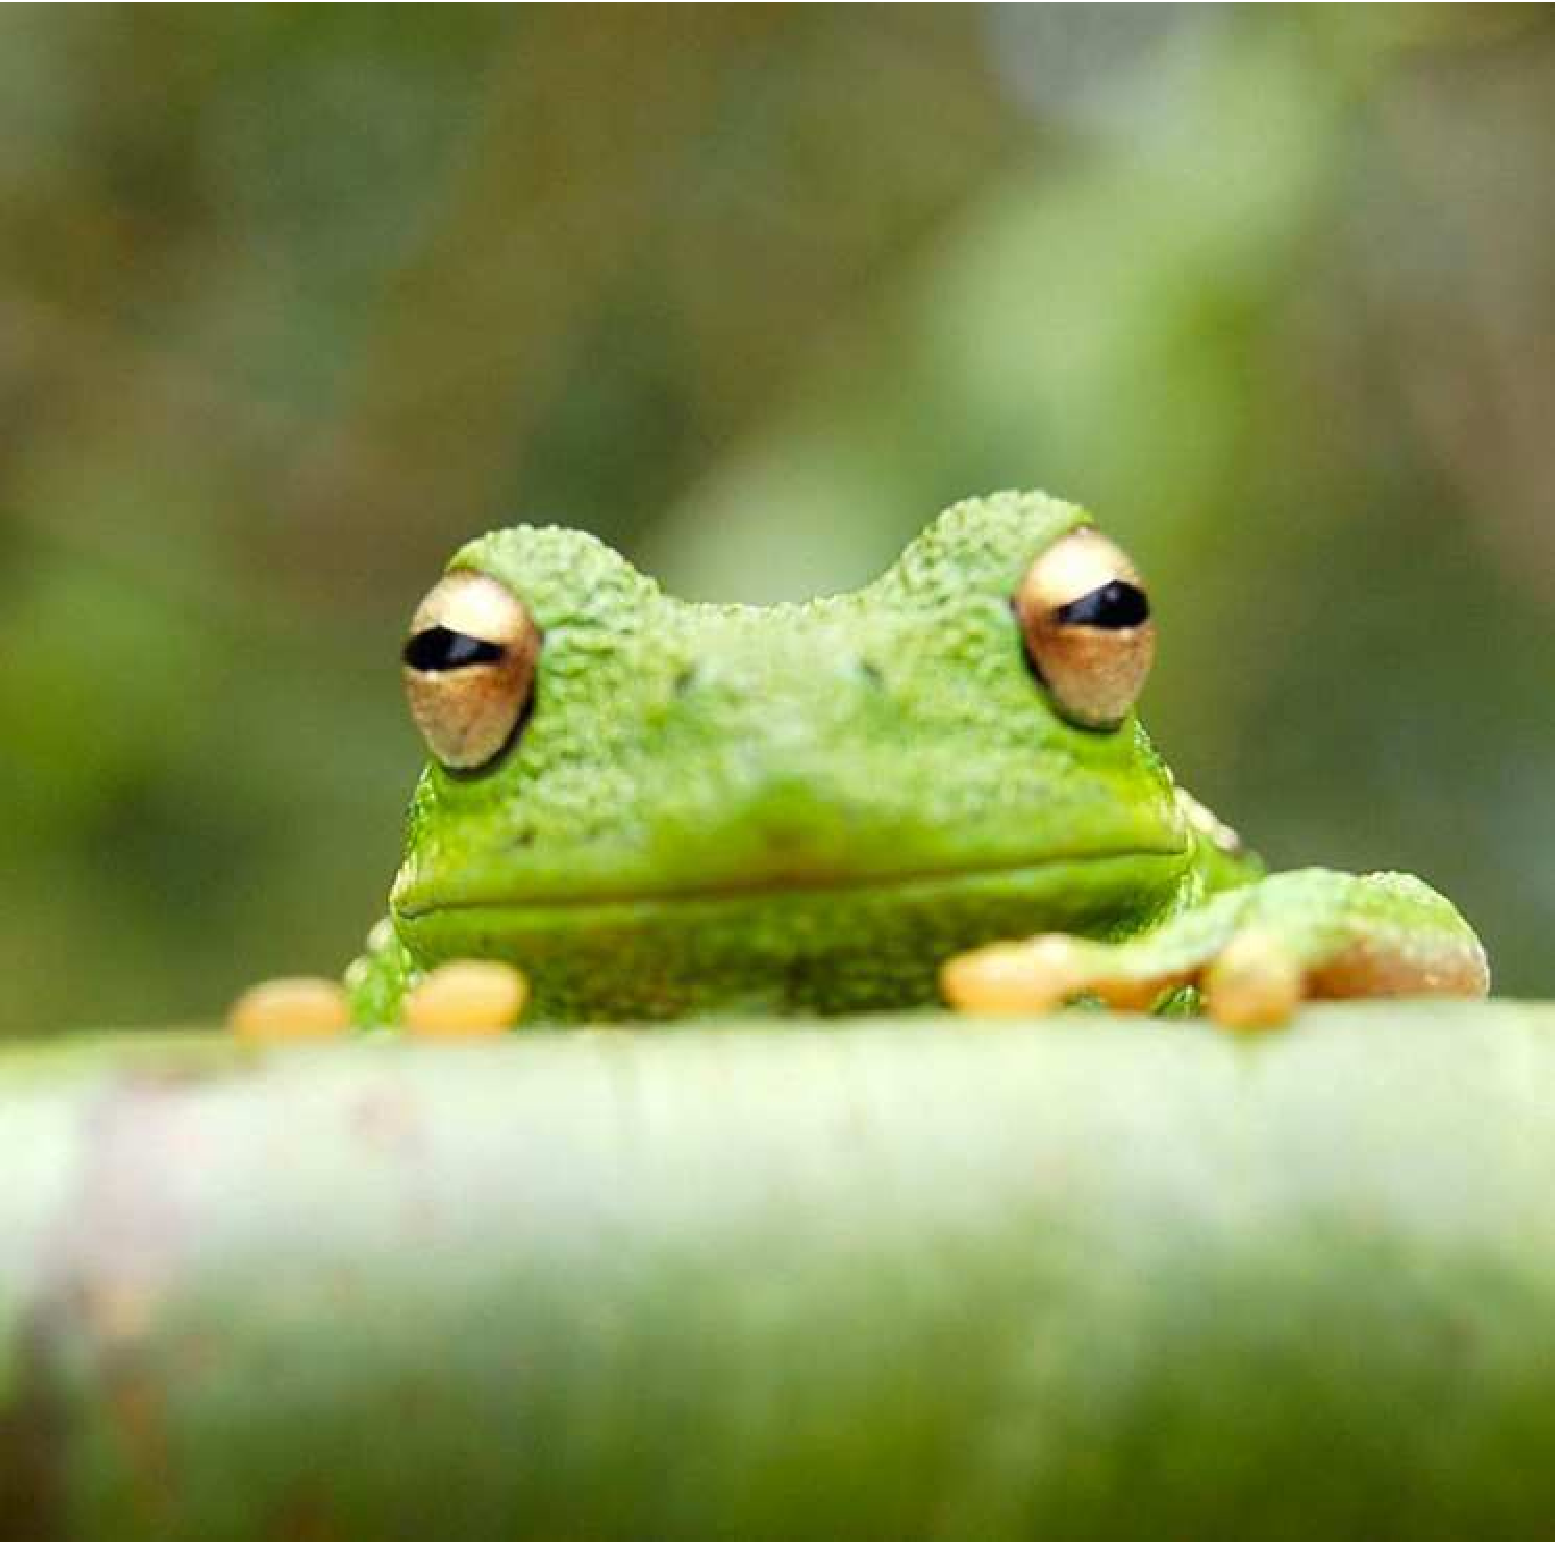
\includegraphics[width=.8\linewidth]{frog.pdf}
% \caption{Placeholder image of a frog with a long example legend to show justification setting.}
% \label{fig:frog}
% \end{figure}



% \begin{table}[t!]
% \centering
% \caption{Comparison of the fitted potential energy surfaces and ab initio benchmark electronic energy calculations}
% \begin{tabular}{lrrr}
% Species & CBS & CV & G3 \\
% \midrule
% 1. Acetaldehyde & 0.0 & 0.0 & 0.0 \\
% 2. Vinyl alcohol & 9.1 & 9.6 & 13.5 \\
% 3. Hydroxyethylidene & 50.8 & 51.2 & 54.0\\
% \bottomrule
% \end{tabular}

% \addtabletext{nomenclature for the TSs refers to the numbered species in the table.}
% \end{table}


% \subsection*{Digital Figures}

% EPS, high-resolution PDF, and PowerPoint are preferred formats for figures that will be used in the main manuscript. Authors may submit PRC or U3D files for 3D images; these must be accompanied by 2D representations in TIFF, EPS, or high-resolution PDF format. Color images must be in RGB (red, green, blue) mode. Include the font files for any text.

% Images must be provided at final size, preferably 1 column width (8.7cm). Figures wider than 1 column should be sized to 11.4cm or 17.8cm wide. Numbers, letters, and symbols should be no smaller than 6 points (2mm) and no larger than 12 points (6mm) after reduction and must be consistent.

% Figures and tables should be labelled and referenced in the standard way using the \verb|\label{}| and \verb|\ref{}| commands.

% Figure \ref{fig:frog} shows an example of how to insert a column-wide figure. To insert a figure wider than one column, please use the \verb|\begin{figure*}...\end{figure*}| environment. Figures wider than one column should be sized to 11.4 cm or 17.8 cm wide. Use \verb|\begin{SCfigure*}...\end{SCfigure*}| for a wide figure with side legends.

\dropcap{A}fter the SARS pandemic in 2005, researchers noted that disease transmission
was not homogeneous: some small number of infected individuals –
"super spreaders" – were responsible for a disproportionately large number of
total infections \cite{nature2005}. Subsequent research noted a similar pattern in
other diseases: between 15\% to 20\% of individuals cased 75\% to 85\% of infections
in diseases as diverse as measles, smallpox, monkeypox, HIV and others
\cite{dimensionsOfSuperspreading}. The COVID-19 pandemic follows a similar pattern:
transmission is dominated by superspreading events (SSEs) in which a 
superspreading individual infects many people over a short time
\cite{plos2020} \cite{nature2021}.

To address this missing piece, we introduce the risk structured "hot-spot"
susceptible-infected-recovered (hsSIR) model, which gives each individual
in a population a probability of spending time in a single "hot-spot" location
where disease spreads more readily. These probabilities are fixed for each individual
over the course of the simulation. The distribution of these risk probabilities
introduces a risk structure to the population and allows us to investigate how
different distributions of risk taking affect the dynamics and outcomes of
a disease outbreak. We find that, compared to the standard SIR model, a small
number of initial infections is less likely to lead to a large outbreak  – in
agreement with SSE theory [@plos2020]. But when large outbreaks do occur they
tend to infect the highest risk individuals early and are more explosive;
peaking faster and often higher than the base model. We also find the decline
in case numbers is faster than would otherwise be expected, as the pool of high
risk individuals is exhausted early; which leads in many cases to a smaller
number of total infections over the entire course of the outbreak. We
corroborate and provide theoretical bases for these findings through the
introduction of a branching process model and an integrodifferential model.


\section*{Agent Based hsSIR Model}

We develop an agent-based model in which N individuals in a fixed population
are susceptible (S), infected (I) or recovered (R) (Fig 1). Each day, each
infected agent may transmit an infection to any susceptible agent with fixed
probability $\beta_C$ (homogeneous community spread – Fig 1Aiii). At the same
time, each agent independently visits the "hot spot" with probability $\rho_i$;
then disease spreads from each infected individual in the hot spot to each
susceptible individual there with probability $\beta_R$ (hot spot spread –
Fig 1Aiii). $\rho_i$ is fixed for each individual but varies between individuals,
we consider different distributions of risk across the population and different
levels of $\beta_R$ and $\beta_C$ (Fig 1B).

Individuals recover from infection after a fixed number of days $D$. We start
each simulation by choosing one individual at random to be infected, and
continue until all agents are either susceptible or recovered.

[Introduce calculated quantities, and cite the table here.]


\section*{Results}

\subsection*{Large Outbreaks Less Likely}

If one person in a small population or community becomes infected, they have a
chance of recovering before spreading the disease to anyone else; or spreading
to only a small number who themselves recover before the initial infection
becomes an outbreak. On the other hand, as soon as more than a very small
number of secondary infections happen, a larger outbreak is all but guaranteed.
This probability of a large outbreak as a result of one initial
infection is a well known function of the population size and infectiousness of
a disease and can be quantified accurately as the probability of disease extinction
of a branching process model (See [@any epidemiology textbook], or
[supplementary explanation/reader of this]).
Existing understanding of super spreading events suggests that increased
heterogeneity in disease spread decreases the probability of a large
outbreak[@nature2005][@eventBasedModel2006].


Our hot spot model confirms this understanding (Figure 2). 
As we increased the relative contribution of hot spot to homogeneous spread in
our model, we found lower probability of a large outbreak. Comparing scenarios
with the same $R_0$ and proportion of hot spot spread, we
found that populations with a lower mean riskiness saw smaller probabilities of
disease outbreak (Figure 2 - lines of different color diverge) –
in these scenarios risk is more heavily concentrated in a smaller portion of the
population so the scenario is more heterogeneous.
Surprisingly, we found that the variance of the distribution of riskiness
across the population plays no role (Figure 2 - lines of different
texture are indistinguishable).

To better understand predicted outbreak probabilities, we follow
[@any epidemiology textbook], [@nature2005] and [@eventBasedModel2006] and
compare the results of the hot spot model to a branching process approximation
in which we compute the probability of disease extinction. In [methods/appendix], 
we show that the extinction probability $\tau$ can be expressed as:

$$\tau = \bar\rho [(1 - \bar\rho \beta_r)(1 - \beta_c) + 
				(1 - (1 - \bar\rho \beta_r)(1 - \beta_c) \tau]^N + 
   (1 - \bar\rho)[(1 - \beta_c) + \beta_c \tau]^N\\$$


\subsection*{Outbreak Sizes Increased for Small $R_0$; Decreased for Large $R_0$}
\subsection*{Dynamics Driven by Rise and Fall of $R_t$}


\matmethods{Please describe your materials and methods here. This can be more
than one paragraph, and may contain subsections and equations as required.

\subsection*{Subsection for Method}
Example text for subsection.
}

\showmatmethods{} % Display the Materials and Methods section

\acknow{Please include your acknowledgments here, set in a single paragraph.
Please do not include any acknowledgments in the Supporting Information,
or anywhere else in the manuscript.}

\showacknow{} % Display the acknowledgments section


\bibsplit[2]
%Use \bibsplit to split the references from the body of the text. Value "[2]" represents the number of reference in the left column (Note: Please avoid single column figures & tables on this page.)

% Bibliography
\bibliography{refs}

\end{document}
